\section{Introdução} \label{sec:intro}

Este trabalho teve como objetivo a implementação de técnicas de pontilhado com difusão de erros. A ideia é reduzir a quantidade de cores tentando manter a imagem o mais próximo possível da original. Isso é feito reduzindo a intesidade para seu limite mais próximo, ao longo de um caminho pela imagem, mas aplicando uma distribuição de erros na vizinhança do pixel.

A \cref{fig:base} apresenta as imagens base deste trabalho, usadas para análise e discussão das formas diferentes de aplicar o pontilhado. As figuras \ref{fig:baboon} e \ref{fig:peppers} são $512 \times 512$, enquanto a \cref{fig:monalisa} é $256 \times 256$ e a \cref{fig:watch} é $1024 \times 768$. Ao todo serão aplicadas 6 distribuições de erro com \red{2 curvas} diferentes em cada figura. As distribuições de erros serão apresentadas ao longo do relatório, na \cref{sec:distribuicoes}, equanto as curvas de varrimento podem ser encontradas na \cref{sec:varredura}.

\begin{figure}[H]
    \centering
    \begin{subfigure}{0.33\textwidth}
    \centering
    \includegraphics[width=4.4cm]{imagens/baboon.png}
    \caption{\texttt{imagens/baboon.png}}
    \label{fig:baboon}
\end{subfigure}%
\begin{subfigure}{0.33\textwidth}
    \centering
    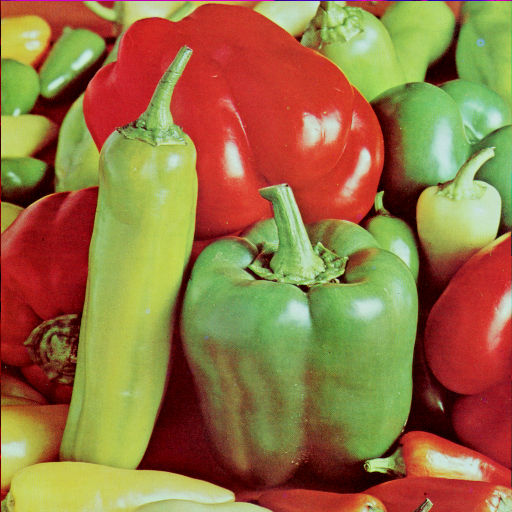
\includegraphics[width=4.4cm]{imagens/peppers.png}
    \caption{\texttt{imagens/peppers.png}}
    \label{fig:peppers}
\end{subfigure}\\[8pt]
\begin{subfigure}{0.33\textwidth}
    \centering
    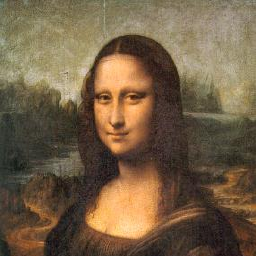
\includegraphics[width=4.4cm]{imagens/monalisa.png}
    \caption{\texttt{imagens/monalisa.png}}
    \label{fig:monalisa}
\end{subfigure}%
\begin{subfigure}{0.33\textwidth}
    \centering
    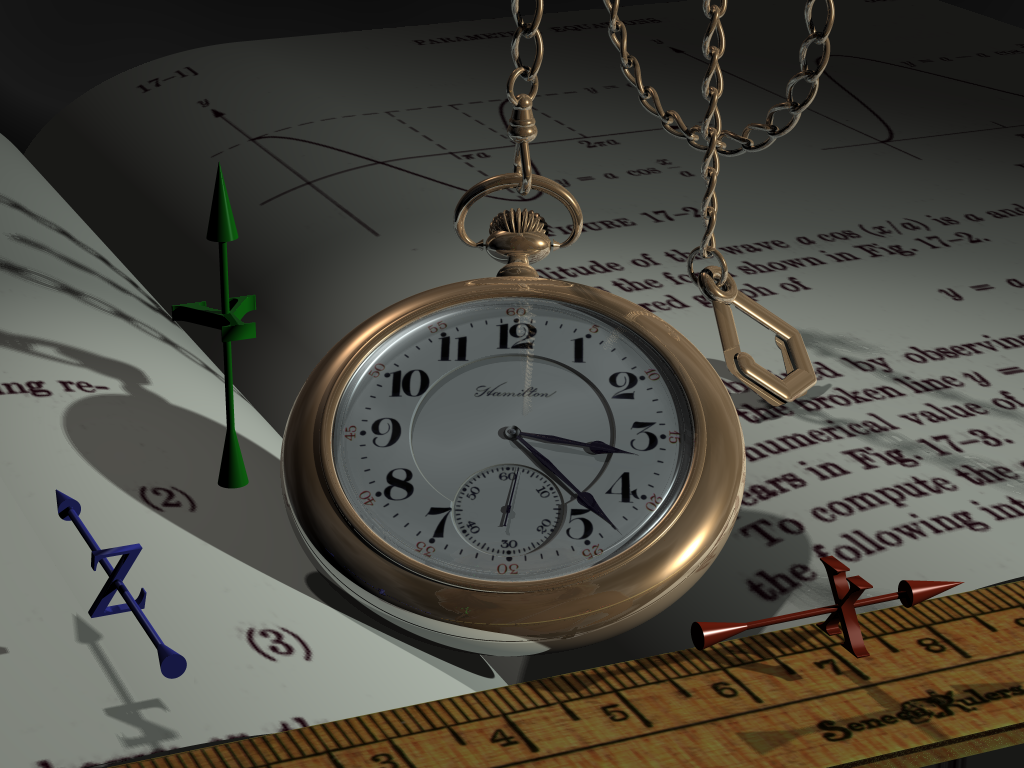
\includegraphics[width=4.4cm]{imagens/watch.png}
    \caption{\texttt{imagens/watch.png}}
    \label{fig:watch}
\end{subfigure}

    \caption{Imagens base da comparação dos filtros.}
    \label{fig:base}
\end{figure}
